\scanpage{3}\mspage{I}
% L1
Soit $H=(S,A,R)$ un hexagone combinatoire

\figure{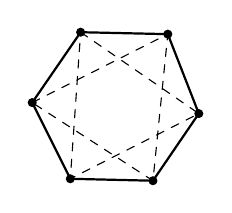
\begin{tikzpicture}[line cap=round,line join=round,scale=.82]
\coordinate (a) at (-.70,1.16); \coordinate (b) at (.65,1.13);
\coordinate (c) at (1.13,-.10); \coordinate (d) at (.42,-1.14);
\coordinate (e) at (-.86,-1.11); \coordinate (f) at (-1.45,.07);
\draw[thick] (a)--(b)--(c)--(d)--(e)--(f)--cycle;
\draw[dashed] (a)--(c)--(e)--cycle (f)--(b)--(d)--cycle;
\foreach \v in {a,b,c,d,e,f}{\fill (\v) circle (2pt);}
\end{tikzpicture}}

% L2–6
Il lui correspond

a) $\omega_H\in\mathrm{Ens}_2$ \unsure{l'ens|l'une} des deux orientations

b) Un torseur $S$ sous $\deleted{\unsure{\mathbb Z/6\mathbb Z\wedge\omega_H|\mathbb Z/6\mathbb Z\wedge\omega_H\simeq}\;\unsure{\mathbb Z/3\mathbb Z\wedge\omega_H}}$
\[
\mathbb Z/6\mathbb Z\wedge\omega_H \simeq
(\mathbb Z/3\mathbb Z\wedge\omega_H)\times
\underbrace{(\mathbb Z/2\mathbb Z\wedge\omega_H)}_{\mathbb Z/2\mathbb Z}
\]
ou ce qui revient au $=$, une paire de deux torseurs.

% L7–10
b$_1$) Un torseur sous $(\mathbb Z/3\mathbb Z\wedge\omega_H)$ i.e. un \deleted{tri} élément
\[
\left\{\begin{aligned}
&\Delta\in\mathrm{Ens}_3\quad\text{avec iso}\\
&\omega_\Delta\simeq\omega_H
\end{aligned}\right.
\]
\margin{\uline{NB} a) et b$_1$) \unsure{équiv. à|équivaut à} : la donnée de $\Delta\in\mathrm{Ens}_3$}
% slanted
\margin{Le groupoïde des hexagones combinatoires est équivalent à la catégorie $(\mathrm{Ens})_3\times(\mathrm{Ens})_2$}
b$_2$) un ens $\unsure{\tau|T}$ à deux éléments

% L11–19
Alors $\Delta$ s'interprète comme l'ens des \deleted{\unsure{deux}}\inserted{trois} diagonales\unsure{,} de $H$, et $\tau$ comme l'ens des deux triangles inscrits. On récupère $\deleted{H}S$ par un iso. can.
\[
S\simeq\Delta\times\tau
\]
(un sommet est connu quand on connaît le triangle inscrit et la diagonale \unsure{que il|qu'il} détermine, et inversement, ceux-ci peuvent être donnés arbitrairement -- )

% L20–22
Notons que cette décomposition implique
\[
S\simeq\coprod_{i\in\tau}S_i\qquad\text{avec}\quad
\begin{aligned}
&\operatorname{card}\tau=2\\
&\operatorname{card}S_i=3\qquad\forall i\in\tau
\end{aligned}
\]
% archive sheet number: 2

